\section{Evaluation}\label{sec:evaluation}

This section discusses the evaluation of the migrated Pastèque implementation with the LLVM-backend in comparison to the original Pastèque implementation targeting Standard-ML \cite{pac-2024} and the efficient Pacheck \cite{pac-2024} checker written in C++.

As the main benchmark, I use the experimental data presented on the original webpage \cite{pacheck_pasteque} for the evaluation.
The dataset consists of different multiplier circuits with different bit-widths, ranging from 32-bit multipliers to 512-bit multipliers.
I use the current version of the AMulet tool by Kaufmann \cite{amulet2} that decides the given multipliers to be correct and also generates proof certificates in the PAC format.
The resulting certificates are then checked by Pastèque with both the LLVM and SML backend and by Pacheck.
I measure wall-clock time and peak RSS for all checkers using GNU time \cite{gnutime}.
Benchmarks are run on a machine with a AMD Ryzen 5 7500F CPU and 32 GB of RAM.
Each benchmark is run five times, the shown measurements are the respective mean values over all five runs.

% Generated by render-table.py from averages.csv.
% Regenerate rather than edit; needs booktabs.
\begin{table}[htbp]
  \centering
  \caption{Wall clock time (\emph{wct}, in seconds) and peak resident set size (\emph{rss}, in MiB) of the three PAC proof checkers. Each value is the mean over 3 rounds. For each benchmark the lower of the two Pastèque backends is set in bold.}
  \label{tab:checker-comparison}
  \begin{tabular}{l rr rr rr}
    \toprule
    & \multicolumn{2}{c}{Pacheck} & \multicolumn{2}{c}{Pastèque LLVM} & \multicolumn{2}{c}{Pastèque SML} \\
    \cmidrule(lr){2-3} \cmidrule(lr){4-5} \cmidrule(lr){6-7}
    Benchmark & wct & rss & wct & rss & wct & rss \\
    \midrule
    128\_128\_U\_SP\_AR\_RC\_GenMul & 1.02 & 138.3 & \textbf{3.10} & \textbf{1045.0} & 5.47 & 2244.6 \\
    256\_256\_U\_SP\_AR\_RC\_GenMul & 5.02 & 544.4 & \textbf{14.03} & \textbf{4226.0} & 22.31 & 15845.1 \\
    512\_512\_U\_SP\_AR\_RC\_GenMul & 21.14 & 2177.9 & 80.50 & 17176.5 & \textbf{64.80} & \textbf{15849.8} \\
    bp-ct-bk-32 & 0.04 & 10.2 & \textbf{0.11} & \textbf{52.2} & 0.24 & 142.8 \\
    bp-wt-cl-32 & 0.04 & 11.1 & \textbf{0.12} & \textbf{56.6} & 0.26 & 141.5 \\
    btor128 & 0.75 & 94.6 & \textbf{2.26} & \textbf{701.7} & 3.78 & 1811.5 \\
    btor256 & 3.83 & 368.6 & \textbf{11.20} & \textbf{2842.5} & 16.49 & 8205.8 \\
    btor512 & 18.09 & 1472.2 & 72.04 & \textbf{11697.5} & \textbf{54.03} & 13601.4 \\
    sp-ar-cl-32 & 0.04 & 12.2 & \textbf{0.14} & \textbf{66.1} & 0.30 & 212.8 \\
    sp-dt-lf-32 & 0.07 & 12.5 & \textbf{0.22} & \textbf{101.2} & 0.47 & 288.7 \\
    \bottomrule
  \end{tabular}
\end{table}

Table \ref{tab:checker-comparison} shows the resulting average measurements.
Between the LLVM backend and the Standard ML backend, the variant with either lower wall clock execution time and memory usage is written in bold, Pacheck is the most efficient for every benchmark.

% Generated by evaluation2/render-plot.py.
\begin{figure}[htbp]
  \centering
  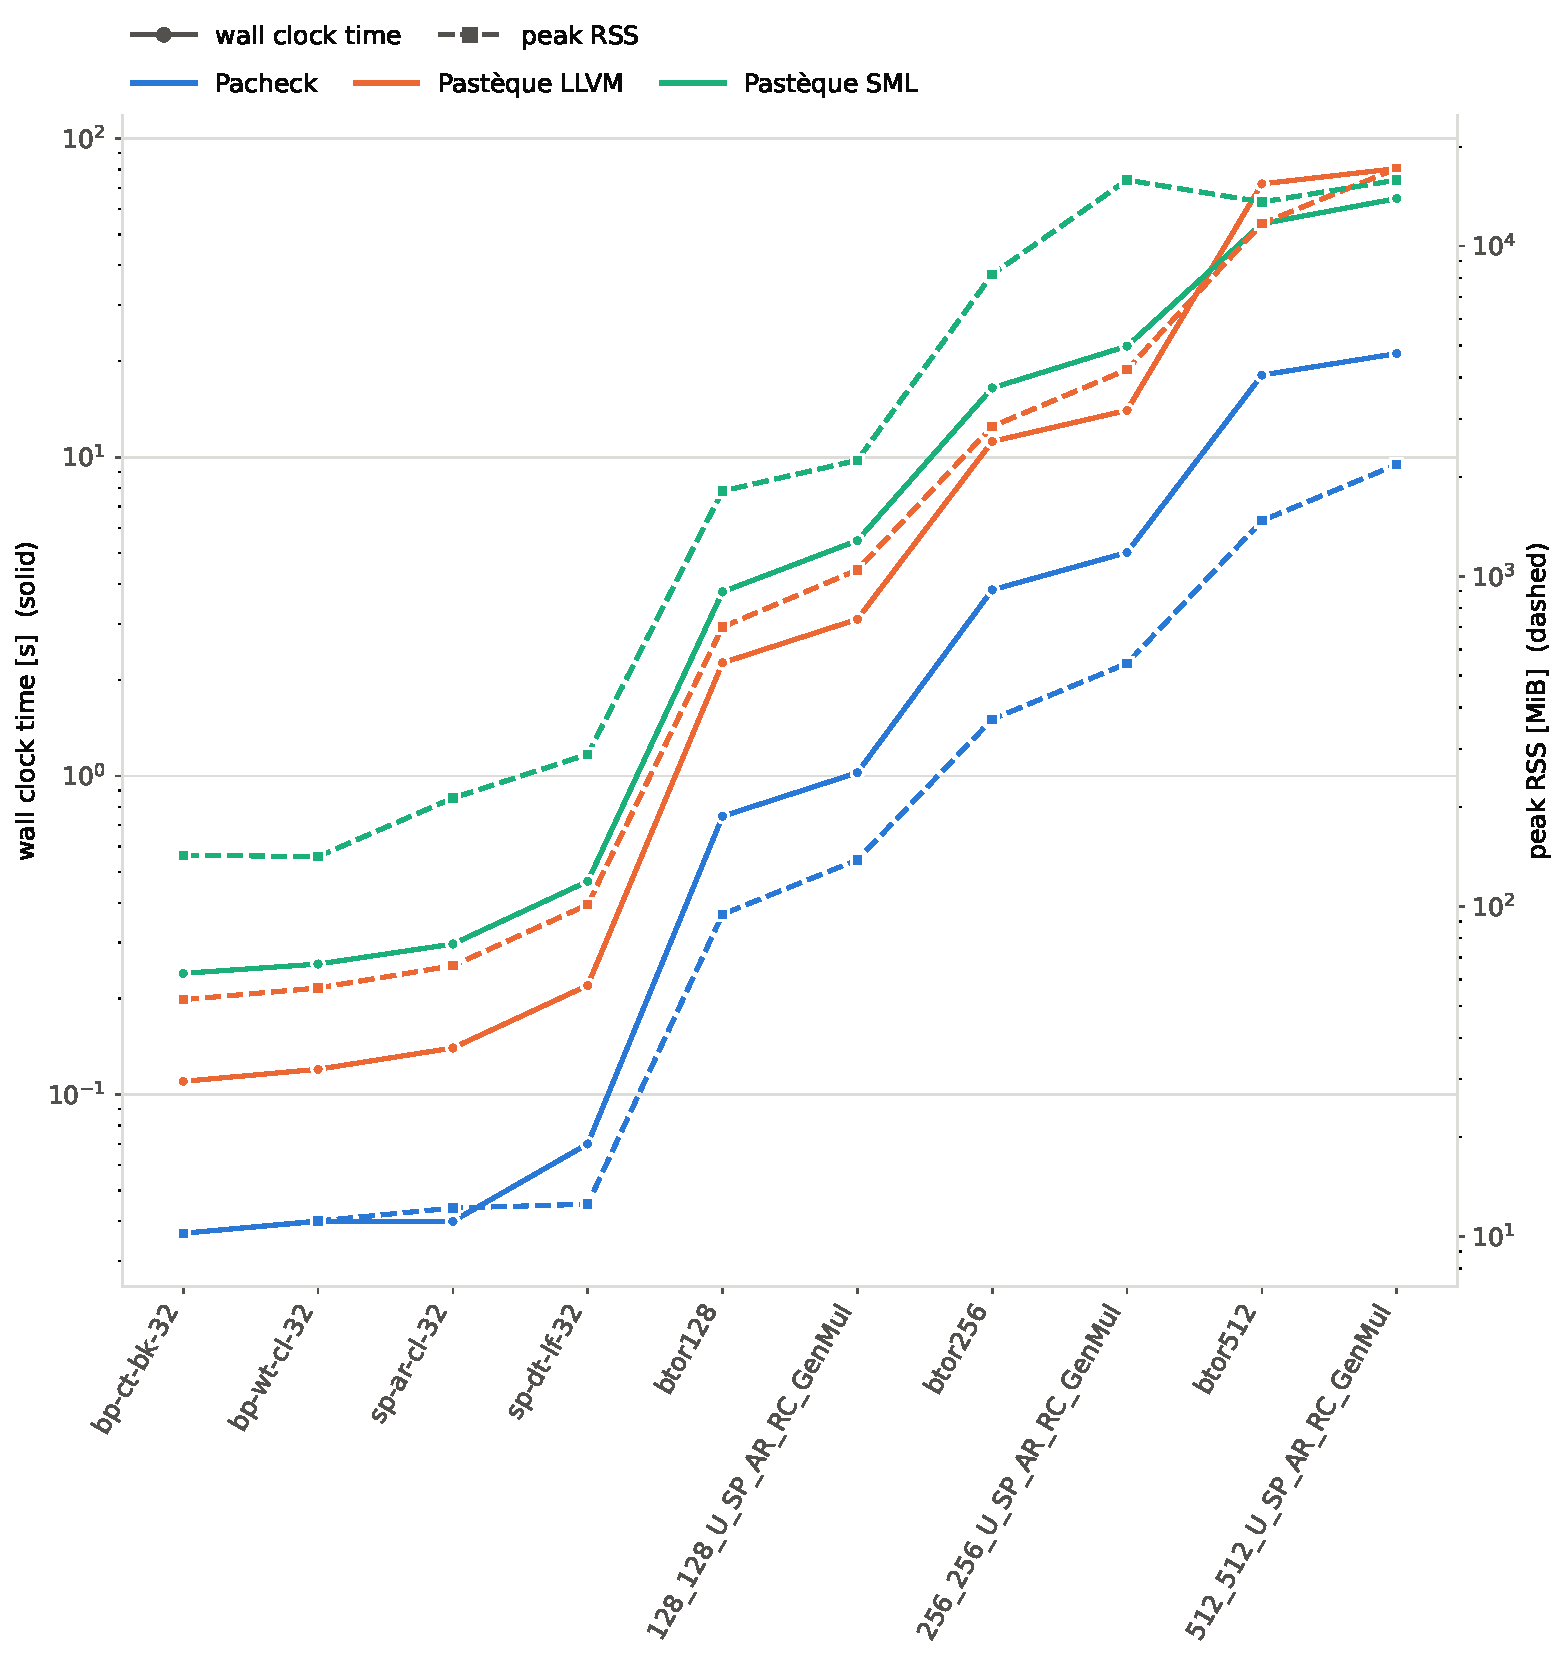
\includegraphics[width=\textwidth]{evaluation2/results/plot.pdf}
  \caption{Wall clock time (solid lines, left axis) and peak resident set size (dashed lines, right axis) of the three PAC proof checkers. Colour identifies the checker, line style identifies the measure. The benchmarks are ordered by the wall clock time of Pastèque with the LLVM backend. Both value axes carry independent scales, so an intersection between a wall clock line and a peak RSS line carries no meaning.}
  \label{fig:checker-comparison}
\end{figure}
